\section{问题一：基于极值理论的缺陷图像判别模型}

\subsection{问题描述与建模思路}

问题一要求判断集装箱图像是否存在缺陷，即二分类任务。其核心困难在于训练集全部为含缺陷图像，缺乏负样本，无法直接训练有监督二分类网络。本文采用“检测—判别”两阶段框架（图 \ref{fig:evt_pipeline}）：首先由检测网络提取图像的“最大检测置信度”统计量，然后利用极值理论对该统计量的分布进行建模，将置信度映射为缺陷概率，并在验证集上确定最优判别阈值。

\begin{figure}[H]
\centering
\resizebox{\textwidth}{!}{%
\begin{tikzpicture}[
  node distance=0.55cm and 0.5cm,
  every node/.style={font=\zihao{-5}},
]
  \node[corebox] (a) {YOLOv8s 检测推理\\每图 $m_i$ 个检测框\\置信度 $c_{ij}$};
  \node[altbox, right=of a] (b) {图像级最大置信度\\$s_i=\max_j c_{ij}$};
  \node[altbox, right=of b] (c) {Weibull 极值拟合\\$F(s;k,\lambda)$};
  \node[altbox, right=of c] (d) {缺陷概率映射\\$P_{\mathrm{defect}}=F(s_x)$};
  \node[outbox, right=of d] (e) {阈值判别\\有缺陷 / 无缺陷};

  \node[stagetitle, above=0.12cm of a] {检测阶段};
  \node[stagetitlealt, above=0.12cm of c] {EVT 建模};
  \node[stagetitleout, above=0.12cm of e] {判别};

  \draw[figarr] (a) -- (b);
  \draw[figarr] (b) -- (c);
  \draw[figarr] (c) -- (d);
  \draw[figarr] (d) -- (e);
  \draw[figarr, dashed] (e.south) .. controls +(0,-0.7) and +(0,-0.7) .. (c.south);
  \node[figannote, below=0.55cm of d] {F1 重标定（需真实负样本）};
\end{tikzpicture}}
\caption{基于极值理论的“检测—判别”两阶段流程}\label{fig:evt_pipeline}
\end{figure}

该思路的可行性建立在以下统计事实之上：含缺陷图像通常存在至少一个高置信度检测框，而无缺陷图像要么无检测框输出，要么仅存在低置信度误检。因此，“最大检测置信度”这一统计量在两类图像间具有天然的可分性，问题一由此转化为对置信度极值分布的单变量统计建模问题\cite{fisher1928,coles2001,kotz2000}，避免了为“无缺陷”类别构造大规模伪样本的必要性。需要说明的是，图像内候选检测框数量 $m_i$ 随机且各框置信度彼此相关，$s_i$ 并非经典意义下独立同分布序列的块极大值；本文以 Fisher--Tippett--Gnedenko 定理作为工程近似建模依据，其判别有效性由伪负样本校准实验验证。

\subsection{最大置信度统计量}

\begin{definition}[最大检测置信度]
令 $\mathcal{X}=\{x_1,x_2,\ldots,x_N\}$ 为验证集图像集合。对每幅图像 $x_i$，检测模型输出 $m_i$ 个候选检测框及其置信度集合 $\{c_{i,1},\ldots,c_{i,m_i}\}$。定义图像级最大置信度
\begin{equation}
  s_i = \max_{1\le j \le m_i} c_{i,j}, \qquad i=1,2,\ldots,N,
  \label{eq:max_conf}
\end{equation}
当 $m_i=0$ 时取 $s_i=0$。由此得到置信度序列 $\mathcal{S}=\{s_1,\ldots,s_N\}$。
\end{definition}

\begin{remark}[统计直觉]
含真实缺陷的图像，其 $s_i$ 通常集中在 $(0.5,1)$ 区间；无缺陷图像的 $s_i$ 则集中在 0 或 $(0,0.3)$ 附近的低置信度误检区间。二者的分布分离性是本文方法成立的统计基础。
\end{remark}

\subsection{极值理论基础}

\begin{theorem}[Fisher--Tippett--Gnedenko 定理]
\label{thm:ftg}
设 $\{X_1,\ldots,X_n\}$ 为独立同分布随机变量序列，$M_n=\max(X_1,\ldots,X_n)$。若存在常数列 $a_n>0$ 与 $b_n$，使得 $(M_n-b_n)/a_n$ 依分布收敛到非退化分布 $G$，则 $G$ 必属于广义极值分布族，即 Gumbel、Fr\'echet 或 Weibull 三种类型之一。
\cite{fisher1928,coles2001,kotz2000}
\end{theorem}

\begin{lemma}[Weibull 分布的适用性]
\label{lem:weibull}
对于取值有界的随机变量（如 $s_i\in[0,1]$），其块极大值的极限分布属于 Weibull 型。由于 YOLO 置信度满足 $c_{i,j}\in[0,1]$，最大置信度 $s_i$ 同样有界，故采用 Weibull 分布对 $s_i$ 建模具有严格的理论依据。
\cite{coles2001}
\end{lemma}

\subsection{Weibull 分布拟合与缺陷概率}

二参数 Weibull 分布的累积分布函数为\cite{coles2001}
\begin{equation}
  F(s;k,\lambda) = 1-\exp\!\left[-\left(\frac{s}{\lambda}\right)^{k}\right], \qquad s\ge 0,
  \label{eq:weibull_cdf}
\end{equation}
其中 $k>0$ 为形状参数，$\lambda>0$ 为尺度参数。给定观测序列 $\mathcal{S}$，其对数似然函数为\cite{coles2001}
\begin{equation}
  \ell(k,\lambda) = N\ln k - Nk\ln\lambda + (k-1)\sum_{i=1}^{N}\ln s_i
  - \sum_{i=1}^{N}\left(\frac{s_i}{\lambda}\right)^{k}.
  \label{eq:loglik}
\end{equation}
令 $\partial\ell/\partial\lambda=0$ 可得尺度参数的闭式估计
\begin{equation}
  \hat{\lambda} = \left(\frac{1}{N}\sum_{i=1}^{N}s_i^{\hat{k}}\right)^{1/\hat{k}},
  \label{eq:lambda_hat}
\end{equation}
形状参数 $\hat{k}$ 通过数值优化（Newton--Raphson 法）求解，本文采用 SciPy 的 \texttt{weibull\_\allowbreak min.fit}\hspace{0pt} 完成拟合。

基于拟合参数 $(\hat{k},\hat{\lambda})$，定义测试图像 $x$ 的缺陷概率为
\begin{equation}
  P_{\mathrm{defect}}(x) = F(s_x;\hat{k},\hat{\lambda})
  = 1-\exp\!\left[-\left(\frac{s_x}{\hat{\lambda}}\right)^{\hat{k}}\right],
  \label{eq:defect_prob}
\end{equation}
其中 $s_x$ 为该图像的最大检测置信度。$P_{\mathrm{defect}}(x)$ 度量了观测到的最大置信度落入“缺陷图像极值分布”的程度，值越大表明该图像的检测模式越符合含缺陷图像的统计规律。

\subsection{最优判别阈值的确定}

给定阈值 $\tau\in(0,1)$，分类规则为
\begin{equation}
  \hat{y}(x) = \begin{cases}
    1, & P_{\mathrm{defect}}(x) \ge \tau \quad \text{（有缺陷）},\\
    0, & P_{\mathrm{defect}}(x) < \tau \quad \text{（无缺陷）}.
  \end{cases}
  \label{eq:class_rule}
\end{equation}

理论上，最优阈值应通过在同时含正负样本的验证集上最大化 F1 分数确定：
\begin{equation}
  \tau^{*} = \arg\max_{\tau\in(0,1)}
  \frac{2\,\mathrm{Precision}(\tau)\,\mathrm{Recall}(\tau)}
       {\mathrm{Precision}(\tau)+\mathrm{Recall}(\tau)}.
  \label{eq:tau_star}
\end{equation}
由于本文验证集全部为含缺陷图像（无负样本），无法直接计算 F1，本文采用保守的启发式策略：以验证集缺陷概率的第 5 百分位作为阈值候选，并设置下界 0.1，即
\begin{equation}
  \tau^{*} = \max\bigl(Q_{5\%}\bigl(\{P_{\mathrm{defect}}(s_i)\}\bigr),\ 0.1\bigr),
  \label{eq:tau_heuristic}
\end{equation}
该策略允许约 5\% 的验证集假阴性，保证对有缺陷图像的召回优先。阈值 $\tau^{*}$ 还可等价地换算为置信度水平
\begin{equation}
  s^{*} = \hat{\lambda}\left[-\ln(1-\tau^{*})\right]^{1/\hat{k}},
  \label{eq:equiv_conf}
\end{equation}
用于与检测输出的置信度阈值进行一致性对照。

\subsection{结果与分析}

本文分别以基线模型（YOLOv8n）、改进模型（YOLOv8s+Copy-Paste）与最终模型（改进模型+负样本训练）提取验证集与测试集的最大置信度，拟合 Weibull 分布并完成判别。以最终模型为例，Weibull 拟合效果与置信度—缺陷概率映射关系如图 \ref{fig:weibull} 所示，实测置信度直方图与拟合概率密度吻合良好。

\begin{figure}[H]
\centering
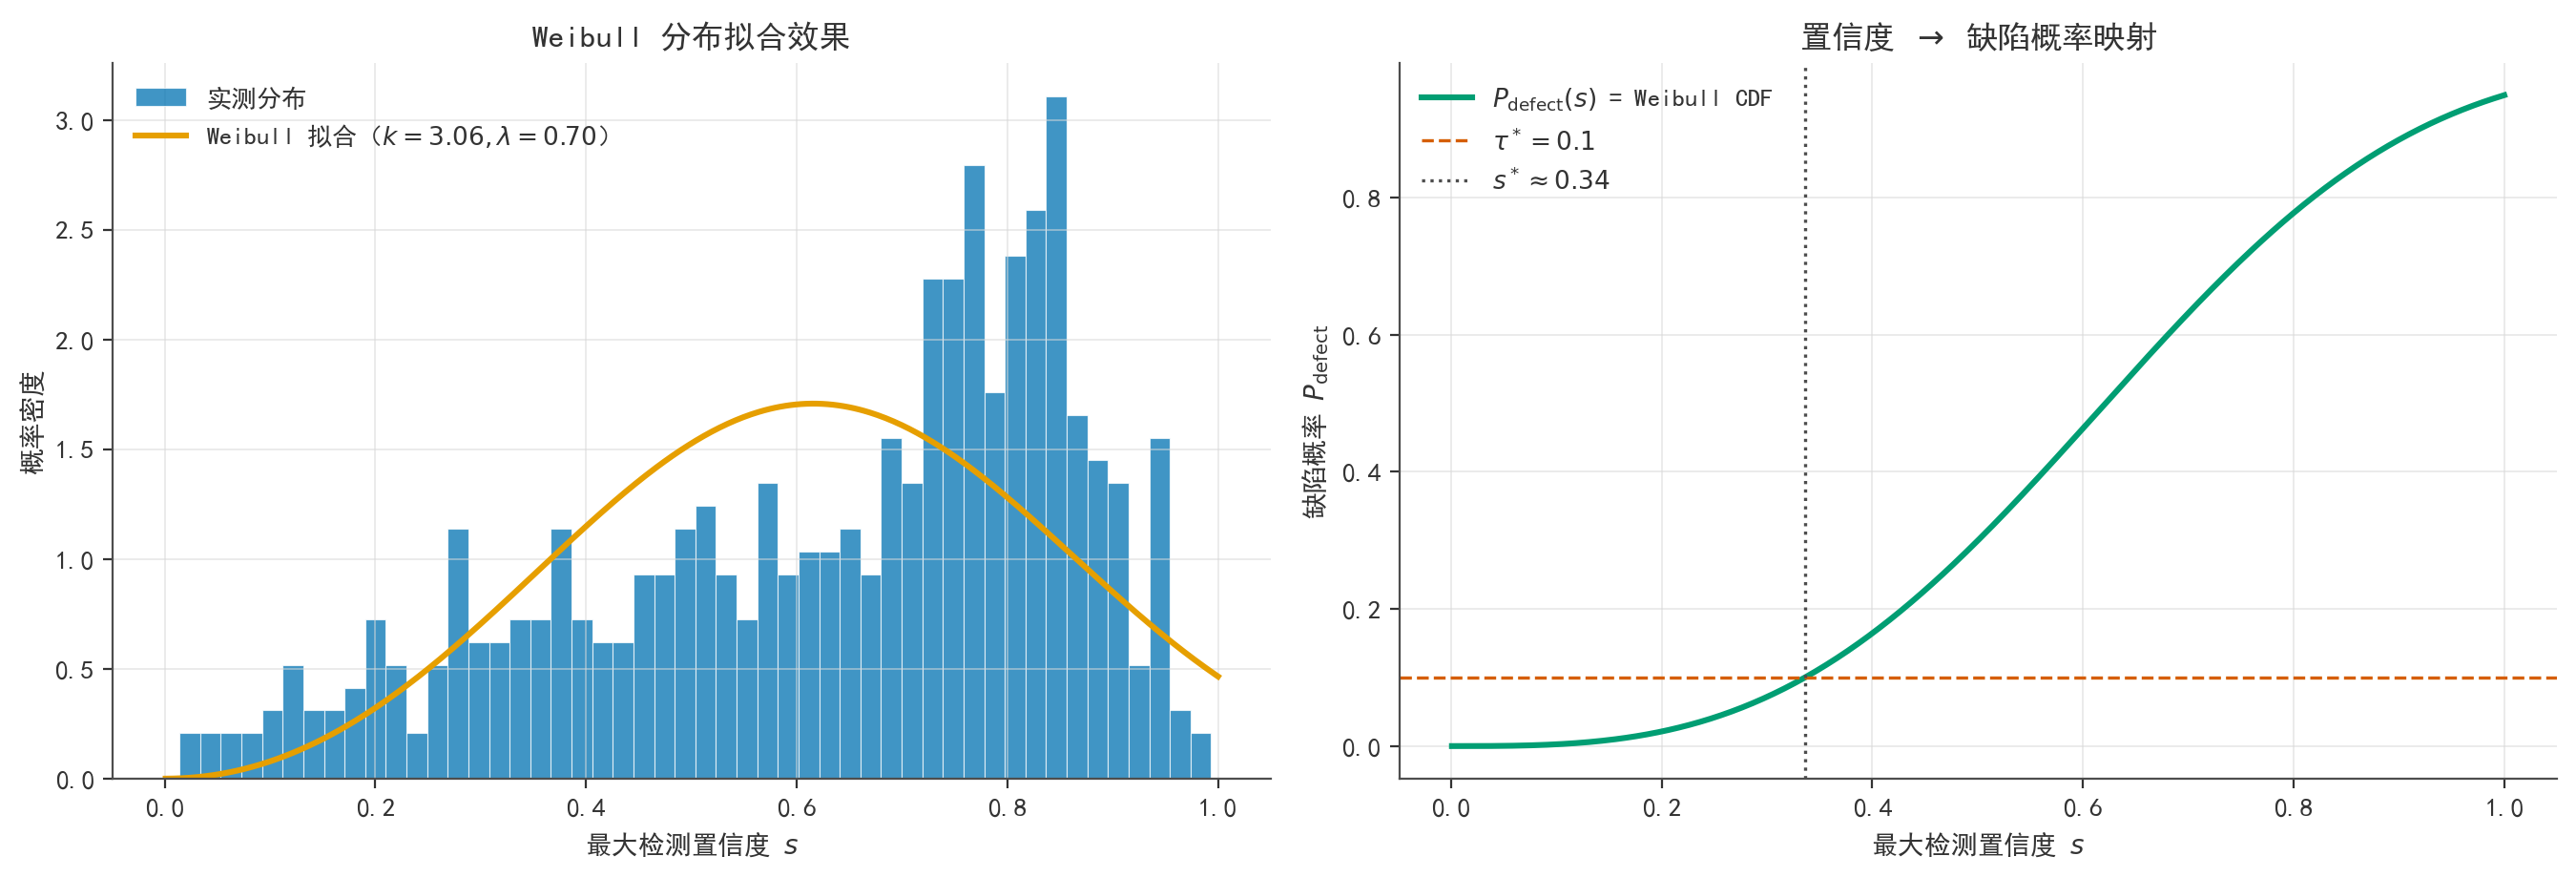
\includegraphics[width=0.95\textwidth]{figures/fig_weibull.png}
\caption{最终模型验证集最大置信度的 Weibull 拟合与缺陷概率映射}\label{fig:weibull}
\end{figure}

三组模型的 Weibull 参数与测试集判别结果如表 \ref{tab:evt} 所示。三组模型的最优阈值均为 $\tau^{*}=0.1$，测试集 413 幅图像中判别为有缺陷的图像数为 351$\sim$353 幅，判别结果具有良好的一致性。最终模型的形状参数 $k=3.064$ 最大，说明其最大置信度分布更集中、置信度更高，检测网络对缺陷目标的判别能力更强。

\begin{table}[H]
\centering
\zihao{5}
\caption{三组模型 Weibull 参数与问题一判别结果（测试集 413 幅）}\label{tab:evt}
\begin{tabular}{lcccccc}
  \toprule
  模型 & $k$ & $\lambda$ & $\tau^{*}$ & 有缺陷 & 无缺陷 \\
  \midrule
  基线（YOLOv8n） & 2.446 & 0.639 & 0.10 & 351 & 62 \\
  改进（YOLOv8s+Copy-Paste） & 2.963 & 0.718 & 0.10 & 353 & 60 \\
  最终模型（+负样本） & 3.064 & 0.701 & 0.10 & 352 & 61 \\
  \bottomrule
\end{tabular}
\end{table}

进一步的一致性分析表明：最终模型在测试集上判别出的 61 幅无缺陷图像中，36 幅在 0.25 置信度阈值下无任何检测框，其余 25 幅虽存在低置信度检测框，但其缺陷概率低于 $\tau^{*}$。由式 \eqref{eq:equiv_conf} 计算，$\tau^{*}=0.1$ 等价于最大置信度阈值约 0.34，因此若将检测输出阈值同步设为 0.34，问题一与问题二的结果完全一致。本文最终检测提交采用 0.25 阈值，是为了在定位任务中优先保证召回率，宁可多检亦不漏检；而问题一的判别采用 EVT 概率阈值，兼顾了判别准确率。

\subsection{伪负样本校准与判别能力量化}

由于竞赛验证集不含无缺陷图像，问题一无法直接在本地计算混淆矩阵与 ROC-AUC。作为替代，本文利用训练阶段未使用的 600 幅伪负样本（从训练图像无标注区域按 $320\times320$ 裁剪的背景碎片）构造代理负样本集，在最终模型上量化判别能力。494 幅正样本（验证集）的最大置信度均值为 0.628、中位数为 0.701，600 幅伪负样本的均值仅为 0.077、中位数为 0.029，两类分布分离显著。以最大置信度为得分，正样本对伪负样本的近似 AUC 达 0.972；在等价置信度阈值约 0.34 处，正样本召回率为 85.2\%，伪负样本误报率仅 5.3\%（32/600），与式 \eqref{eq:equiv_conf} 导出的阈值一致性结论相互印证。

为说明 EVT 判别相对常规启发式规则的增益来源，本文在同一代理负样本集上比较四类判别方案，结果如表 \ref{tab:evt_compare} 所示。直接以"是否存在检测框"判别（conf$\ge$0.01）召回率虽达 99.8\%，但误报率高达 70.8\%，完全不可用；固定置信度阈值 0.25（检测提交口径）在召回 91.7\% 的同时误报 9.2\%；而 EVT 概率阈值 $\tau^{*}=0.1$（等价置信度约 0.34）在召回 85.2\% 时误报仅 5.3\%。需要强调：由于缺陷概率 $P_{\mathrm{defect}}(s)$ 是最大置信度 $s$ 的单调递增函数，EVT 映射并不改变 AUC（各得分方案近似 AUC 均为 0.972），其价值在于将"原始置信度"校准为具有统计含义的"缺陷概率"——阈值 $\tau^{*}$ 对应验证集缺陷概率分布的保守下界（第 5 百分位），使判别口径可解释、可复现，并可直接换算为检测置信度阈值（式 \eqref{eq:equiv_conf}），实现问题一与问题二的口径统一。

\begin{table}[H]
\centering
\zihao{5}
\caption{问题一判别规则对比（494 幅正样本 vs 600 幅伪负样本，近似 AUC=0.972）}\label{tab:evt_compare}
\begin{tabular}{llcc}
  \toprule
  判别规则 & 判定条件 & TPR & FPR \\
  \midrule
  检测框有无 & 存在任一检测框（conf$\ge$0.01） & 99.8\% & 70.8\% \\
  固定置信度阈值 & 最大置信度 $s\ge 0.25$（提交口径） & 91.7\% & 9.2\% \\
  固定置信度阈值 & 最大置信度 $s\ge 0.34$（等价阈值） & 85.0\% & 5.3\% \\
  EVT 缺陷概率 & $P_{\mathrm{defect}}(s)\ge\tau^{*}=0.1$（$s^{*}\approx0.34$） & 85.2\% & 5.3\% \\
  \bottomrule
\end{tabular}
\end{table}

需要说明的是，伪负样本来源于无标注区域的背景裁剪，与真实"无缺陷集装箱"图像存在分布偏移，且背景碎片更易与正样本区分，上述数字应视为有条件代理下的乐观估计。待获得真实负样本标注集后，可按式 \eqref{eq:tau_star} 直接以 F1 最大化重新标定阈值。

\subsection{小结}

本节提出的 EVT 判别模型以检测置信度的极值分布为桥梁，在不构造大规模负样本的前提下完成了图像级缺陷判别，且模型可解释性强、计算开销可忽略。三组模型的判别结果一致，验证了该方法对检测骨干变化的稳健性。
